% Document inspired by: https://www.overleaf.com/latex/templates/business-card-template/yrqjgydpprrb

\documentclass[10pt]{article}
\usepackage[dvips]{graphicx}
%\graphicspath{ {../Images} }
\usepackage[utf8]{inputenc}
\usepackage[T1]{fontenc}
\usepackage{xcolor}
\usepackage{tikz}

\usepackage{geometry}
\geometry{total={210mm,297mm},hmargin=10mm,vmargin=2mm}

\pagestyle{empty}

\renewcommand\familydefault{\sfdefault}
\usepackage{tgadventor}

% Setting buisness card size
\newlength{\cardw}
\newlength{\cardh}
\setlength{\cardw}{85mm}
\setlength{\cardh}{55mm}

\begin{document}
	
	\begin{tikzpicture}
		% grid
		\foreach \i in {0,1,2,3,4,5} \draw[very thin, gray,dashed] (0,\i*\cardh) -- (2*\cardw,\i*\cardh);
		\foreach \j in {0,1,2} \draw[very thin, gray,dashed] (\j*\cardw,0) -- (\j*\cardw,5*\cardh);
		% card content
		\foreach \i in {0,1} \foreach \j in {0,1,2,3,4} {
			
			\node at (\i*\cardw+0.2\cardw,\j*\cardh+0.5\cardh) {
\includegraphics[width=0.3\cardw]{site_qrcode.png}};

			\node[black!25!gray] at (\i*\cardw+0.50\cardw,\j*\cardh+0.85\cardh) {\Large \textbf{Francesco Rombaldoni}};
			
			\node at (\i*\cardw+0.53\cardw,\j*\cardh+0.65\cardh) {\textbf{Riversamenti}};
			\node at (\i*\cardw+0.53\cardw,\j*\cardh+0.59\cardh) {\textbf{di filmati}};
			\node at (\i*\cardw+0.53\cardw,\j*\cardh+0.53\cardh) {\textbf{analogici}};
			\node at (\i*\cardw+0.53\cardw,\j*\cardh+0.47\cardh) {\textbf{in digitale}};
			\node at (\i*\cardw+0.50\cardw,\j*\cardh+0.2\cardh) {-Tel-};
			\node at (\i*\cardw+0.50\cardw,\j*\cardh+0.1\cardh) {f.rombaldoni@campus.uniurb.it};
			
			\node at (\i*\cardw+0.85\cardw,\j*\cardh+0.5\cardh) {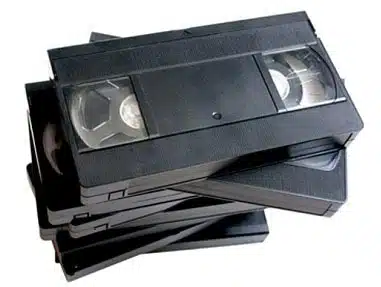
\includegraphics[width=0.27\cardw]{VHS.png}};
		};
	\end{tikzpicture}
	
\end{document}